Como se mencionó en la introducción, la privacidad del voto es fundamental legalmente al proceso electoral. El mayor riesgo es la unificación de un registro de voto con un registro de votante.
El quiebre de la confidencialidad del voto significa que alguien sepa qué es lo que otra persona votó. Es importante evitar que esto sea posible para que cada ciudadano se pueda sentir libre de votar a quién quiera sin presiones. De poder averiguarlo, otras personas podrían tomar represalias o tratar de comprar votos de la población para su conveniencia. Los votos podrían averiguarse en dos instancias: mientras el ciudadno está votando, o a posteriori desde la memoria del aparato o el lugar donde los resultados se almacenaran.
%De igual forma que en Estándares de almacenamiento de votos, mencionaremos distintas técnicas que se utilizaron en distintos países, y los agujeros de seguridad que se encontraron en tales.

\subsection{Identificación del votante a partir de registros}

En todos los sistemas que se analizaron para este trabajo donde se guardan los registros de los votantes, éstos van por separado al voto en sí mismo, para proteger la confidencialidad. Pero si hubiera forma de unir ambas listas, esa seguridad se ve comprometida.

Un ejemplo es Brasil, donde se optó por dejar de utilizar VVPAT debido al incremento del costo por las impresoras y por problemas operacionales. En su lugar, se adoptó un sustituto totalmente digital. Los votos pasaron a almacenarse en una estructura de datos llamada DRV (Digital Record of the Vote) en la memoria electrónica de la maquina de votación. Esta estructura es una tabla separada en secciones, donde cada sección está dedicada a una postulación distinta. Para que no se pueda saber quién voto a quién, esta tabla almacena en distinto orden en que fueron emitidos los votos (La tabla shufflea los votos emitidos)\cite{aranha}.
DRV fue introducido como un reemplazo de VVPAT permitiendo una verificación independiente de los resultados de la elección. Sin embargo, VVPAT es independiente de los votos computados electrónicamente a diferencia de DRV ya que este último es producido por la misma pieza de software que los cuenta. De esta forma, cualquier ataque exitoso al proceso de contar los votos, compromete la integridad de la DRV.

\begin{figure}[H]
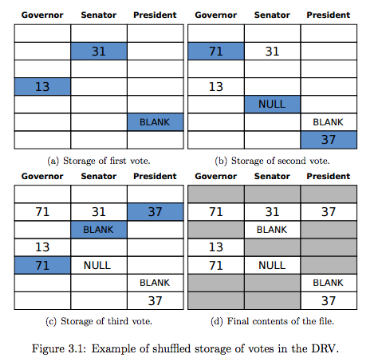
\includegraphics[width=0.5\textwidth]{Imagenes/privacidad1}
\caption{Ejemplo de votos en DRV}
\end{figure}

La ilustración anterior es un ejemplo de una votación utilizando la estructura de datos DRV, donde
\begin{enumerate}
	\item El primer elector vota a la opción 13 como gobernador, a la 31 como senador, y deja el voto en blanco para presidente
	\item El segundo elector vota a la opción 71 como gobernador, impugna su voto para senador, y vota a la opcion 37 como presidente
	\item El tercer y último elector, vota a la opción 71 como gobernador, deja en blanco la de senador y a la opcion 37 como presidente
\end{enumerate}

Se encontraron tres vulnerabilidades:
\begin{enumerate}
	\item Una inadecuada elección del generador de números pseudo-aleatorios. Se utilizan las funciones rand y srand de C que tienen un período muy corto y aceptan solo semillas de 32 bits.
	\item Mala elección de la semilla. La semilla es el horario de apertura de la mesa de votación, que es durante las 7AM y 8AM, dando tan solo 3600 posibilidades.
	\item Semilla pública. No sólo que el proceso de elección de la semilla es determinística, sino que también se la publica en la documentación oficial de la mesa.
\end{enumerate}

Dadas estas vulnerabilidades, se puede realizar los dos siguientes tipos de ataque:
\begin{enumerate}
	\item Ataque directo: Se obtiene la semilla de la documentación oficial de la mesa, y se simula el movimiento de shuffle con N votos y se detecta en qué posición de la DRV fue almacenado cada voto. Esto permite obtener los votos en orden tan solo mirando la documentación oficial. Se pierde el anonimato de la votación si se conoce el orden en que los votantes emitieron sus votos.
	\item Ataque indirecto: Dado los votos fuera de orden, es posible realizar una búsqueda exhaustiva en los posibles valores de semillas, que son 3600, comparando los espacios vacíos.  Con la semilla correcta, se puede realizar el primer ataque
\end{enumerate}

En las EVM en India, existe un ataque que afecta a la privacidad del voto llamado Clip-on Memory Manipulator Attack\cite{india}. A diferencia del ataque mencionado en una sección anterior en el que se intercambia una placa, en este se agrega temporalmente nuevo hardware a la máquina que registra los votos, permitiendo dos ataques: robar votos y violar el secreto del voto.
\begin{figure}[H]
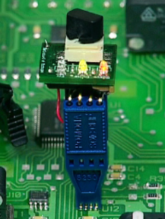
\includegraphics{Imagenes/privacidad2}
\caption{Hardware a agregar. Al girar la perilla, se indica que candidato favorecer}
\end{figure}


\subsection{Acceso ilegítimo al momento de votar}

Este tipo de ataques consisten en averiguar el voto mientras la persona está sufragando. Este tipo de quiebre de confidencialidad es especialmente problemático porque contradice uno de los principales beneficios del voto electrónico que es que la gente con discapacidades visuales o motrices pueda efectuar su voto sin ayuda de otra persona, y por lo tanto, en secreto.

Una de las formas de violar este principio es a través de la lectura de formas de almacenamiento externo, como la BUE en la ciudad de Buenos Aires donde existen dos posibles ataques que comprometen la privacidad del voto\cite{votar}.

El primero es que se pierde el anonimato del voto, ya que el voto se escribe en el chip RFID de una BUE y se puede leer el contenido de estos chip a cierta distancia sin que el votante se entere. No solo eso, sino que también cada chip RFID tiene un número que lo identifica. Por ende, si sabemos el orden en que los electores votan y se les da una BUE con un orden predeterminado podemos, al finalizar, revisar el número del RFID, saber a qué elector pertenece y su voto\cite{smaldone:chip}.

El segundo posible ataque también corresponde a la pérdida del anonimato del voto pero no se utiliza esta vez el chip RFID, sino la memoria EEPROM integrada de 256KB que se encuentran en el microcontrolador ARM. En esta memoria se puede almacenar todo tipo de información, como por ejemplo el voto y una marca de tiempo. Por ende, similar al anterior, con conocer el orden de los electores al votar se puede saber las elecciones de los electores.

Otro ejemplo de lectura posible de los votos en la urna es en el sistema israelí (que es muy parecido al usado en Argentina). Éste se denomina ``relay attack''\cite{oren:2010}\cite{oren:2012}, donde la comunicación con las dos partes es iniciada por el atacante que luego simplemente transmite mensajes entre las dos partes sin manipularlas ni siquiera necesariamente leerlos, hasta obtener su objetivo.

Un ejemplo de un relay attack es que Peggy trabaja en un edificio de alta seguridad que se accede utilizando una tarjeta inteligente en su bolso. Cuando se acerca a la puerta del edificio, el edificio detecta la presencia de una tarjeta inteligente e inicia un intercambio de mensajes para verificar que la tarjeta es de Peggy. El edificio le permite a Peggy entrar. Mallory quiere entrar en el edificio. Mallory se acerca al edificio con un dispositivo que simula una tarjeta inteligente, y el edificio responde iniciando el intercambio de mensajes. Mallory reenvía el mensaje a su cómplice Evelyn que está siguiendo a Peggy mientras hace mandados en otra parte de la ciudad. Evelyn retransmite el mensaje a la tarjeta inteligente de Peggy, escucha la respuesta de la tarjeta inteligente de Peggy, y envía la respuesta a Mallory, que la transmite al edificio. Continuando de esta manera, Mallory y Evelyn transmiten los mensajes entre el edificio y la tarjeta inteligente de Peggy hasta que el edificio esté satisfecho de que se está comunicando con tarjeta inteligente de Peggy. El edificio se abre y entra Mallory.\cite{wiki:relay}

Esta implementación israelí sufre los siguientes ataques:
\begin{itemize}
	\item Ballot sniffing attack, el cual permite leer todos los votos en la urna en cualquier momento. Al realizar este ataque antes de que un elector vote, y acto seguido de que el elector votó sin que nadie más haya votado aún, se puede saber a quién votó el elector afectando el anonimato del voto.
Para realizar este ataque, un retransmisor se establece entre los votos dentro de la urna y la terminal de verificación dentro de la cabina de votación que se encarga de retransmitir el contenido de los votos de la urna a la terminal de verificación para saber su contenido. Se activa repetidamente la terminal de verificación, cada vez con una votó diferente y se almacena su respuesta
\begin{figure}[H]
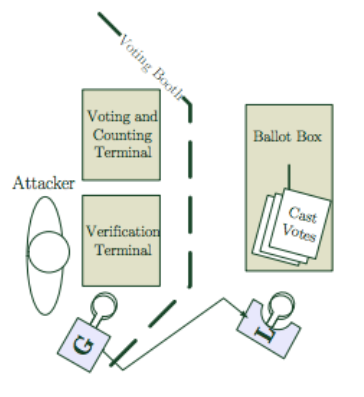
\includegraphics{Imagenes/privacidad3}
\caption{Ballot sniffing attack}
\end{figure}
	\item Single dissident attack, el cual permite suprimir votos.

	\item Zapping attack, el cual permite anular los votos de una urna

	\item Jamming attack, el cual permite interrumpir la operacion de una terminal de voto electronico a distancia

	\item Fault attack, el cual hace que la estación se encuentre en un estado inválido y luego dándola de baja

\end{itemize}

Para los dos primeros ataques, es necesario un retransmisor.

Israel, un país conocido por su desarrollo rápido y continuo de la tecnología, tuvo la oportunidad de poner en práctica el voto electrónico ya en 2008\cite{e-lected}. Sin embargo, a pesar de la aprobación en general de la clase política, esto no sucedió, y en la actualidad el país no lo usa. ¿Por qué? Israel es un ejemplo de los riesgos que corre un país cuando su proceso de modernización electoral no es transparente y abierto a la gente.

En 2008, el Ministerio del Interior israelí publicó una propuesta de ley para la implementación del voto electrónico en los próximos eventos electorales después de una prueba exitosa en paralelo a las elecciones locales de 2007. Sin embargo, esta propuesta plantea dos problemas: en primer lugar, no hubo una discusión pública sobre el asunto, y todo se hizo a puerta cerrada; segundo, las máquinas de votación del país que querían usar no emiten recibos de voto, lo que hizo que el electorado sospechoso de su auditabilidad.

Se demostró que contenía vulnerabilidades, y la falta de medios para auditabilidad .
Al final, tras las protestas de los ciudadanos en tensión, la iniciativa de votación electrónica fue cancelada e Israel tuvo que volver a votación manual.


Por último, y bastante más complicado, está el ejemplo de la auditoría holandesa, donde se logró identificar el voto mientras sucedía a través de un ``side-effect'' muy interesante: la frecuencia de radio\cite{holanda}. En este ataque, se logró encontrar una señal a varias frecuencias distintas, representada como un zumbido, y se dilucidó que la frecuencia cambiaba si el texto a mostrar por pantalla tenía caracteres especiales porque el controlador utilizado para mostrarlos necesitaba hacer más trabajo. En particular, en los Países Bajos al momento de la auditoría uno de los partidos más importantes tenía un caracter acentuado y el otro no, con lo que se podía saber de oído (con cierto aparato para escuchar la frecuencia) por las emisiones de la máquina si un votante elije a cierto partido.

Con un poco más de trabajo, analizando las emisiones irradiadas por la pantalla en más detalle, se pudieron identificar todos los candidatos por separado, pero en la auditoría se aclaraba que ese nivel de trabajo no era factible a ser realizado al momento de la elección estando suficientemente cerca de la máquina.
